% User Guide of SSSI
\documentclass[12pt]{article}
\usepackage[centertags]{amsmath}
\usepackage{amsfonts}
\usepackage{amssymb}
\usepackage{latexsym}
\usepackage{amsthm}
\usepackage{newlfont}
\usepackage{graphicx}
\usepackage{listings}
\usepackage{booktabs}
\usepackage{abstract}
\usepackage{tikz}
\usepackage{caption}
\usepackage{subcaption}
\usepackage{algorithm,algorithmic}
\lstset{numbers=none,language=MATLAB}

\bibliographystyle{amsplain}
\renewcommand{\textfraction}{0.15}
\renewcommand{\topfraction}{0.85}
\renewcommand{\bottomfraction}{0.65}
\renewcommand{\floatpagefraction}{0.60}
%\newcommand{\topfigrule}{%
%  \vspace*{5pt}\hrule\vspace{-5.4pt}}
%\newcommand{\botfigrule}{\vspace*{-5.4pt}\hrule\vspace{5pt}}


\newlength{\defbaselineskip}
\setlength{\defbaselineskip}{\baselineskip}
\newcommand{\setlinespacing}[1]%
           {\setlength{\baselineskip}{#1 \defbaselineskip}}
\newcommand{\doublespacing}{\setlength{\baselineskip}%
                           {2.0 \defbaselineskip}}
\newcommand{\singlespacing}{\setlength{\baselineskip}{\defbaselineskip}}
% MATH -------------------------------------------------------------------
\newcommand{\A}{{\cal A}}
\newcommand{\h}{{\cal H}}
\newcommand{\s}{{\cal S}}
\newcommand{\W}{{\cal W}}
\newcommand{\D}{{\cal D}}
\newcommand{\NN}{\mathbb N}
\newcommand{\BH}{\mathbf B(\cal H)}
\newcommand{\KH}{\cal  K(\cal H)}
\newcommand{\Int}{\mathbb Z}
\newcommand{\Complex}{\mathbb C}
\newcommand{\Field}{\mathbb F}
\newcommand{\RPlus}{[0,\infty)}
\newcommand{\rip}{\operatorname{RIP}}
\newcommand{\pj}{\text{Proj}}
\newcommand{\csp}{\overline{\operatorname{span}}}
\newcommand{\spn}{\operatorname{span}}
%
\newcommand{\norm}[1]{\left\Vert#1\right\Vert}
\newcommand{\essnorm}[1]{\norm{#1}_{\text{\rm\normalshape ess}}}
\newcommand{\abs}[1]{\left\vert#1\right\vert}
\newcommand{\set}[1]{\left\{#1\right\}}
\newcommand{\seq}[1]{\left<#1\right>}
\newcommand{\eps}{\varepsilon}
\newcommand{\To}{\longrightarrow}
\newcommand{\RE}{\operatorname{Re}}
\newcommand{\IM}{\operatorname{Im}}
\newcommand{\supp}{\text{supp}}
\newcommand{\Poly}{{\cal{P}}(E)}
\newcommand{\EssD}{{\cal{D}}}
\newcommand{\argmin}{\operatornamewithlimits{argmin}}
\newcommand{\argmax}{\operatornamewithlimits{argmax}}
\newcommand{\Fc}{\mathcal{F}}
\newcommand{\Ac}{\mathcal{A}}
\newcommand{\Ic}{\mathcal{I}}
\newcommand{\Nc}{\mathcal{N}}
\newcommand{\Ex}{\mathbb{E}}
\newcommand{\real}{\mathbb{R}}
%\newcommand{\Pr}{\textsc{P}}
\newcommand{\cL}{\mathcal{L}}
\newcommand{\cF}{\mathcal{F}}
\newcommand{\Xf}{\mathfrak{X}}
\newcommand{\bx}{\boldsymbol{x}}
\newcommand{\by}{\boldsymbol{y}}
\newcommand{\bw}{\boldsymbol{w}}
\newcommand{\bmu}{\boldsymbol{\mu}}
\newcommand{\bthe}{\boldsymbol{\theta}}
\newcommand{\bA}{\boldsymbol{A}}
\newcommand{\ba}{\boldsymbol{a}}
\newcommand{\bb}{\boldsymbol{b}}
\newcommand{\bd}{\boldsymbol{d}}
\newcommand{\bff}{\boldsymbol{f}}
\newcommand{\bF}{\boldsymbol{F}}
\newcommand{\bp}{\boldsymbol{p}}
\newcommand{\bG}{\boldsymbol{G}}
\newcommand{\bg}{\boldsymbol{g}}
\newcommand{\bh}{\boldsymbol{h}}
\newcommand{\bH}{\boldsymbol{H}}
\newcommand{\bk}{\boldsymbol{k}}
\newcommand{\bL}{\boldsymbol{L}}
\newcommand{\bs}{\boldsymbol{s}}
\newcommand{\bm}{\boldsymbol{m}}
\newcommand{\bn}{\boldsymbol{n}}
\newcommand{\bP}{\boldsymbol{P}}
\newcommand{\bR}{\boldsymbol{R}}
\newcommand{\bI}{\boldsymbol{I}}
\newcommand{\bJ}{\boldsymbol{J}}
\newcommand{\bQ}{\boldsymbol{Q}}
\newcommand{\bU}{\boldsymbol{U}}
\newcommand{\bV}{\boldsymbol{V}}
\newcommand{\bLam}{\boldsymbol{\Lambda}}
\newcommand{\bzero}{\boldsymbol{0}}
\newcommand{\diag}{\mathrm{diag}}
\newcommand{\mymatrix}[1]{\begin{bmatrix} #1\end{bmatrix}}
\newcommand{\comment}[1]{}
\newcommand{\tr}{{\text{tr}}}
\newcommand{\hx}{\hat{\mathbf{x}}}
\newcommand{\hy}{\hat{\mathbf{y}}}
\newcommand{\hz}{\hat{\mathbf{z}}}



% THEOREMS ---------------------------------------------------------------
\theoremstyle{plain}
\newtheorem{thm}{Theorem}[section]
\newtheorem{cor}[thm]{Corollary}
\newtheorem{lem}{Lemma}[section]
\newtheorem{prop}[thm]{Proposition}
%
\theoremstyle{definition}
\newtheorem{defn}{Definition}[section]
\newtheorem{eg}{Example}[section]
%
\theoremstyle{remark}
\newtheorem{rem}{Remark}[section]
%
\numberwithin{equation}{section}
\renewcommand{\theequation}{\thesection.\arabic{equation}}
\newcommand{\ds}{\displaystyle}
\newtheorem{assum}{Assumption}
\newtheorem{them}{Theorem}[section]
\newtheorem{coro}{Corollary}[section]
\begin{document}
\title{User Guide of SSSI}
\author{Entao Liu \thanks{Center for Energy \& Geo Processing (CeGP), School of ECE, Georgia Tech, e-mail: liuentao@gmail.com}
and Lingchen Zhu \thanks{Center for Signal and Information Processing (CSIP), School of ECE, Georgia Tech 
e-mail: lczhu@gatech.edu}} \maketitle

\section{Requirements and License}

SSSI is a Matlab based package. Besides Matlab (2012a or later version recommend), you also need a C++ compiler to generate the mex function. 
SSSI is free for use in academic research. is distributed in the hope that it will be useful, but WITHOUT ANY
WARRANTY. If you find any glitches within the package or you want to share your extensions to SSSI, please contact the authors. We will keep the packages updated and thank you for your contribution. By far, some source files in SSSI are already inherited from other open source package, please read the comments in codes for authorship and contact information. 

\section{Introduction}
The SSSI is designed to provide a package for seismic simulation. The purpose of package is more on the educational side than the performance of the computation. Thus we build the package based on Matlab for the readability of the codes, easy of data visualization, etc. The major functions has been of the package are the following:
\begin{itemize}
\item Acoustic wave simulation for 2D/3D
\item Elastic wave simulation for 2D
\item Kirchhoff's migration
\item Reverse Time Migration (RTM)
\item Full Waveform Inversion (FWI)
\end{itemize}
The purpose of this manual is not to provide a comprehensive review of numerical simulation of wave equation and seismic imaging, but rather guide for you to quickly learn how to use SSSI and what you can do with it. We will only show and explain necessary equations to keep it concise.
Interested users are suggested to read the references therein for details.  

\section{Numerical Simulation of Acoustic Wave}
\subsection{Acoustics wave equation}
The seismic method is one of the basic tools in exploration geophysics. People fire off man-made vibration sources (e.g. dynamite, viborseis trucks, and air gun) then the wave propagates through the subsurface media. The reflection and refraction will be recorded by geophones (on shore) and hydrophones (off shore). In order to simulate this process with computers, it is crucial to simulate the wave propagation in the media
accurately and efficiently. The real earth is an elastic media, such that the seismic waves contain both P-waves and S-waves. For simplicity, we some times only consider a P-wave field, which is mathematically described by an acoustic wave equation. It is verified by borehole data that the media density variations are not the main source of reflected waves. It is reasonable to assume constant density of the media. Then the acoustic wave equation is  
\begin{equation}\label{aw}
\frac{1}{c^2(\bx)}\frac{\partial^2 p(\bx,t)}{\partial t^2}-\Delta p(\bx,t)=f(\bx,t),
\end{equation}
where $p(\bx)$ is the filed of pressure variation and $\bx=(z,x)$ or $\bx=(z,x,y)$ is the coordinates in the Cartesian coordinate system for the 2D and 3D case, respectively. Following the convention in geophysics, the $z$ direction is point downwards. The $c(\bx)$ is the velocity of P-wave at the point $\bx$. The $f_s(\bx,t)$ is the source term. Moreover, $\Delta$ in (\ref{aw}) is the Laplace operator defined as 
\begin{equation}
\Delta: =\left\{
\begin{aligned}
\frac{\partial^2}{\partial x^2}+\frac{\partial^2}{\partial z^2}~~~~~~~ & ~~~~\text{for 2D }\\
\frac{\partial^2}{\partial x^2}+\frac{\partial^2}{\partial y^2}+\frac{\partial^2}{\partial z^2} &~~~~ \text{for 3D}
\end{aligned}
\right.  
\end{equation}

\subsection{Finite Difference Method on Standard Grid}
There are two popular methods of solving the wave equation numerically. One is the Finite Difference Method (FDM), the other is the Finite Elements Method (FEM) method. Each method has its pros and cons. Concretely, the FD method which is adopted by the SSSI is simple to implement. For most of the simulations, its accuracy is enough. The FEM usually provides more accurate results, which is based on adaptive meshing (multiscale) of the simulation region. However, its implementation is less straightforward, especially when adding boundary conditions.   

In order to solve the wave equation with a FDM, functions are represented by their values at certain discrete grid point and and derivatives are approximated through difference in these values. In SSSI, we use the equi-distributed grid points $(z_i)_{0\le i \le I-1 }$, $(x_j)_{0\le j \le J-1}$, and $(t_n)_{0\le n \le N-1}$ given by $z_i = i\Delta z$, $x_j = j\Delta x$ and $t_n=n\Delta t$. Instead of solving the wave equation in a continuous domain (both in space and time) analytically, the FDM looks for a numerical solution on these grid points.  

A crucial step of FDM is to find good approximations of the derivatives in (\ref{aw}) with function values on the grid points. Let us begin with the definition of the derivative, 
 \begin{equation}
  \begin{aligned}
  \frac{\partial p(z, x, t)}{\partial z} &= \lim\limits_{\Delta z \rightarrow 0} \frac{p(z+\Delta z, x, t) - p(z, x, t)}{\Delta z}\\
  &\approx \frac{p(z+\Delta z, x, t) - p(z, x, t)}{\Delta z}.
  \end{aligned}
  \end{equation}
  assuming the finite grid size $\Delta z$ is small enough.
  Apply this approximation twice. We can derive an estimation of the 2nd derivative in (\ref{aw})
  \begin{equation}
  \begin{aligned}
  &\frac{\partial^2 p(z, x, t)}{\partial z^2} = \frac{\partial}{\partial z}\frac{\partial p(z, x, t)}{\partial z} \approx \frac{\frac{\partial p(z, x, t)}{\partial z} - \frac{\partial p(z-\Delta z, x, t)}{\partial z}}{\Delta z}\\
  &\approx \frac{p(z+\Delta z, x, t) - 2p(z, x, t) + p(z-\Delta z, x, t)}{\Delta z^2}.
  \end{aligned}
  \end{equation}
  
For simplicity of the notations, we denote $p_{i,j}^{(n)}:=  p(i\Delta z, j\Delta x, n\Delta t)$, $f_{i,j}^{(n)} := f(i\Delta z, j\Delta x, n\Delta t)$, $v_{i,j} := v(i\Delta z, j\Delta x)$.
 Therefore, a finite difference expression of 2-D acoustic wave equation can be written as 
  \begin{equation}
    \begin{aligned}
    &\frac{1}{v_{i,j}^2}\frac{p_{i,j}^{(n+1)} - 2p_{i,j}^{(n)} + p_{i,j}^{(n-1)}}{\Delta t^2} + f_{i,j}^{(n)} \\
    &= \frac{p_{i+1,j}^{(n)} - 2p_{i,j}^{(n)} + p_{i-1,j}^{(n)}}{\Delta z^2} + \frac{p_{i,j+1}^{(n)} - 2p_{i,j}^{(n)} + p_{i,j-1}^{(n)}}{\Delta x^2}.
    \end{aligned}
  \end{equation}
Simple algebraic manipulations lead to a recursive expression of the wave equation,
  \begin{equation}
    \begin{aligned}
    &p_{i,j}^{(n+1)} = \frac{v_{i,j}^2\Delta t^2}{\Delta z^2}\left(p_{i+1,j}^{(n)} - 2p_{i,j}^{(n)} + p_{i-1,j}^{(n)}\right)\\
    &+ \frac{v_{i,j}^2\Delta t^2}{\Delta x^2}\left(p_{i,j+1}^{(n)} - 2p_{i,j}^{(n)} + p_{i,j-1}^{(n)}\right)\\
    &+ 2p_{i,j}^{(n)}-p_{i,j}^{(n-1)}-v_{i,j}^2\Delta t^2 f_{i,j}^{(n)}.
    \end{aligned}
  \end{equation}
  All values of $p$ are computed on integer grid points as we illustrated in Figure \ref{fig:stanG}. The FDM on standard grid is easy to understand and implement, however it is not adopted in SSSI because of its drawbacks in accuracy.  
  
\begin{figure}
\centering
\begin{subfigure}[b]{.4\textwidth}
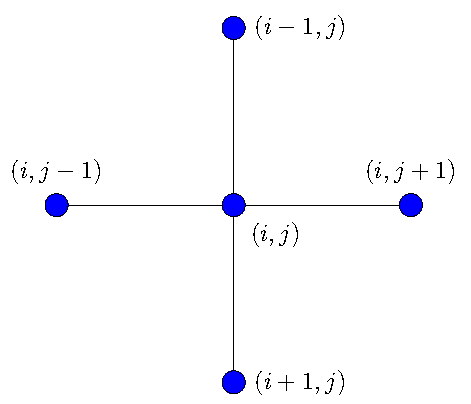
\includegraphics[width=5cm]{Fig/stanGrid}
\caption{Standard Grid.}
\label{fig:stanG}
\end{subfigure}
~~~~~
\begin{subfigure}[b]{0.4\textwidth}
\includegraphics[width=5cm]{Fig/StagGrid}
\caption{Staggerd Grid.}
\label{fig:stagG}
\end{subfigure}
\caption{Discretization grids.}
\end{figure}

\subsection{Finite Difference Method on Staggered Grid}
With a sophisticated design, we can actually obtain higher order of approximation of the derivatives if we have access to the value of $p$ on the half grid points, as denoted by the green dots in Figure \ref{fig:stagG}. 

By Taylor expansion of a function $p(u)$ on the half grid points, where $u = z, x; \; k = 0, 1, 2, \dots $
  \begin{equation}\label{half1}
      p\left(u + \frac{2k+1}{2}\Delta u\right) = p(u) + \sum\limits_{n=1}^{\infty} \frac{1}{n!}\frac{\partial^n p(u)}{\partial u^n}\left(\frac{2k+1}{2}\Delta u\right)^n 
      \end{equation}
      \begin{equation}\label{half2}
      p\left(u - \frac{2k+1}{2}\Delta u\right) = p(u) + \sum\limits_{n=1}^{\infty} \frac{(-1)^n}{n!}\frac{\partial^n p(u)}{\partial u^n}\left(\frac{2k+1}{2}\Delta u\right)^n
  \end{equation}
  Take the difference between (\ref{half1}) and (\ref{half2}). It cancels all the terms when $n$ is even.
So it implies for $k = 0, 1, 2, \dots$
\begin{equation}    \label{Fdiff}
    \begin{aligned}
   &  \frac{p\left(u + \frac{2k+1}{2}\Delta u\right) - p\left(u - \frac{2k+1}{2}\Delta u\right)}{(2k+1)\Delta u}\\
    &~~~~~~~~~  =  \frac{\partial p(u)}{\partial u} + \sum\limits_{n=1 }^{\infty} \frac{1}{(2n+1)!}\frac{\partial^{(2n+1)} p(u)}{\partial u^{(2n+1)}}\left(\frac{2k+1}{2}\Delta u\right)^{2n}.
    \end{aligned}
    \end{equation}
We can approximate $\frac{\partial p(u)}{\partial u}$ as a weighted sum of finite difference in (\ref{Fdiff})
  \begin{equation}\label{weight}
  \begin{aligned}
    &\frac{\partial p(u)}{\partial u} = \sum\limits_{k=0}^{N-1} a_k \frac{p\left(u + \frac{2k+1}{2}\Delta u\right) - p\left(u - \frac{2k+1}{2}\Delta u\right)}{(2k+1)\Delta u} \\
    &= \sum\limits_{k=0}^{N-1} a_k \left[ \frac{\partial p(u)}{\partial u} + \frac{\Delta u^2}{3! \cdot 2^2}(2k+1)^2\frac{\partial^3 p(u)}{\partial u^3} \right.\\&\left. + \frac{\Delta u^4}{5! \cdot 2^4}(2k+1)^4\frac{\partial^5 p(u)}{\partial u^5} + \cdots \right.\\&\left. + \frac{\Delta u^{2N-2}}{(2N-1)! \cdot 2^{2N-2}}(2k+1)^{2N-2}\frac{\partial^{2N-1} p(u)}{\partial u^{2N-1}} + o(\Delta u^{2N}) \right].
  \end{aligned}
  \end{equation}
If the weighted $\{ a_k\}_{k=0}^{N-1}$ are chosen carefully, we can eliminate all the term on the right hand side of (\ref{weight}) and make the coefficient of $\frac{\partial p(u)}{\partial u} =1$. These $N$ weights generate a approximation of the derivative of order $2N$ 

Solving $\{a_k\}_{k=0}^{N-1}$ by the following linear equations
\begin{equation*}
\begin{bmatrix}
  1 & 1 & \cdots & 1 \\
  1^2 & 3^2 & \cdots & (2N-1)^2 \\
  1^4 & 3^4 & \cdots & (2N-1)^4 \\
  \vdots & \vdots & \ddots & \vdots \\
  1^{2N-2} & 3^{2N-2} & \cdots & (2N-1)^{2N-2} \\
\end{bmatrix}
\begin{bmatrix}
  a_0 \\ a_1 \\ a_2 \\ \vdots \\ a_{N-1}
\end{bmatrix}
=
\begin{bmatrix}
  1 \\ 0 \\ 0 \\ \vdots \\ 0
\end{bmatrix}
\end{equation*}
\begin{equation*}
  \begin{aligned}
  N = 1&: a_0 = 1\\
  N = 2&: a_0 = 9/8, a_1 = -1/24\\
  N = 3&: a_0 = 75/64, a_1 = -25/384, a_2 = 3/640\\
  &\vdots
  \end{aligned}
\end{equation*}

The source code which generates the appropriate weights can be found at \texttt{src/dCoef.m}. Moreover, the finite difference operator is fulfilled by \texttt{src/diffOperator.m}. 


\subsection{Absorbing Boundary Conditions (ABC)}
For the sake of efficiency and storage, we only simulate wave propagation in a truncated region which contains the seismic source and array of sensors. In a real seismic survey, the seismic wave generated by the source should have no reflection on the boundaries to mimic the unbounded media. If we do not care with particular techniques, the numerical simulation will generate strong reflections on the boundaries which do not exist in the real earth. A widely adopted method is to impose the absorbing boundary conditions (ABC), in order to attenuate the reflections. In the 2D scenario, we pad the left, right, bottom boundaries with absorbing boundaries of certain width (fulfilled by \texttt{src/extBoundary.m}). The wave will be attenuated in those absorbing boundaries and keep unaltered out side of the absorbing boundaries. Throughout the SSSI, except specified explicitly, we consider the top of the simulated region to be the surface of the earth to be a free surface and do not apply absorbing boundary to it.


\begin{figure}
\centering
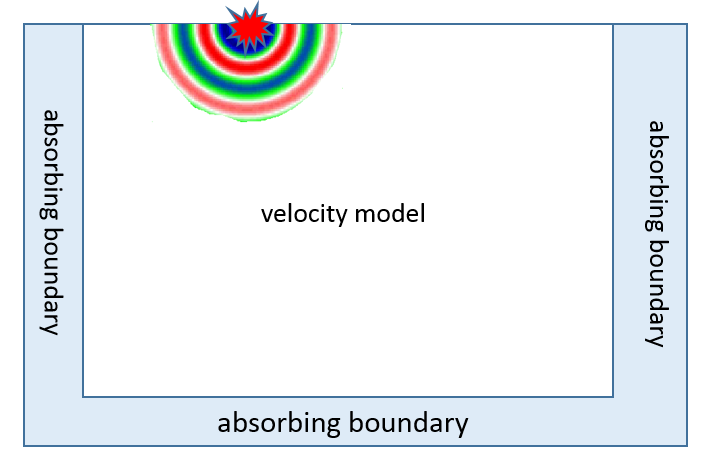
\includegraphics[width=0.6\textwidth]{Fig/abc.png}
\caption{Absorbing boundaries of the 2D simulation region}
\end{figure}

\subsubsection{Sponge ABC}
Numerically, the simple method for the ABC is called sponge ABC \cite{CerKosAO1985}. Suggested by its name, the reflections are exponentially attenuated in the extended artificial boundary area by multiplying a factor $d(u) < 1$.
\begin{equation}
  d(u) = e^{-\alpha^2\text{dist}(u)^2}, \mbox{  where  } u=x, z
\end{equation}
where $\text{dist}(u)$ is the distance from $u$ to the original boundary in the $u$ direction. 

The source code of which implements the acoustic wave propagation with sponge ABC 
is \texttt{src/fwdTimeSpongeFor2dAw.m}. Through out all names of the source files in SSSI,  we follow this rule: \texttt{fwd} means forward (\texttt{rvs} means reverse); \texttt{Time} means the equation is solved in the time domain (\texttt{freq} means in frequency domain); \texttt{For2d} means 2 dimensional (\texttt{For3d} means 3 dimensional); and \texttt{Aw} is short
 for acoustic wave (\texttt{Ew} is for elastic wave). 
 
\begin{figure}
\centering
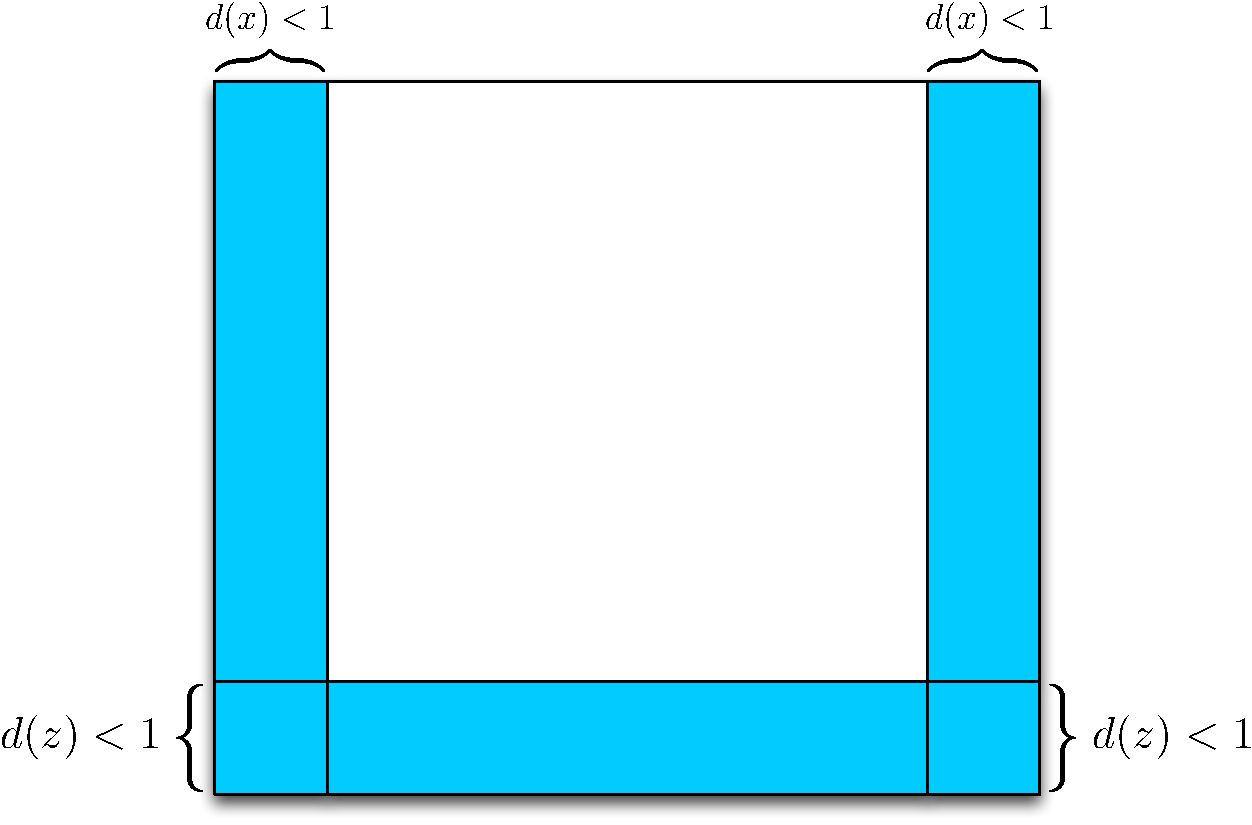
\includegraphics[width=0.7\textwidth]{Fig/SpongeABC.pdf}
\caption{Sponge ABC}
\end{figure}


\subsubsection{Perfectly Matched Layer (PML)}
 Perfectly Matched Layer (PML) method which was originally formulated for use with Electromagnetic equations outperforms other existing methods. It is proven to be efficient for wave equations (both acoustic and elastic) as well \cite{KomMar2007}. The PML have a zero reflection coefficient for all angles of incidence and all frequencies before discretization. Moreover, a PML interface between a physical medium and the extended artificial boundary completely absorbs incident waves from the physical medium regardless of its incidence angle and frequency.
By defining a damping profile $d(u)$ ($u=z, x, y$) function (see \texttt{src/dampPml.m}) such that $d(u) = 0$ inside the physical medium and $d(u) > 0$ in the PML region, a new complex coordinate $\tilde{u}$ is introduced as
  \begin{equation}\label{replace}
  \tilde{u}(u) = u + \frac{1}{j\omega}\int_0^u d(s)\mathrm{d}s.
  \end{equation}
Or equivalently,
  \begin{equation}
  \frac{\partial}{\partial \tilde{u}} = \frac{j\omega}{j\omega + d(u)}\frac{\partial}{\partial u} = s_u(j\omega)\frac{\partial}{\partial u}.
  \end{equation}
In the homogeneous media, the acoustic wave equation has the following solution $A \exp(-j (\bk \cdot \bx -\omega t))$, where $A$ represents the amplitude and polarization of the plane wave. The $\bk = k_x \hx + k_y \hy +k_z \hz$ denotes the wave vector, which 
indicates the direction of wave propagation of the plane wave. $\bx = x\hx +y\hy +z \hz$ is the position vector. After the replacement in (\ref{replace}), we can derive another solution of the acoustic equation as follows,
\begin{equation}
\begin{aligned}
&A\exp(-j(k_x \tilde{x} + k_y y + k_z z -\omega t))=\\
 &~~~~~~~~~~~~A\exp(-j (\bk\cdot \bx -\omega t))\exp(-kx/\omega \int_0^x d(s)ds).
\end{aligned}
\end{equation}
In the original simulated region the the new solution is equivalent to the old one, since $d_x=0$. Additionally, in the $\hat{\mathbf{n}}= \hx$ direction, the wave amplitude decay with a coefficient $\exp(-kx/\omega \int_0^x d(s)ds)$ that is inversely proportional to the angular frequency $\omega$ of the plane wave. 

In SSSI we use a non-split method, the Convolutional PML (CPML) \cite{LueHun1992, RodGed2000, KomMar2007}, which is more reasonable to work with the acoustic (pressure) source. In time domain,
  \begin{equation}
    \frac{\partial}{\partial \tilde{u}} = s_u(t) * \frac{\partial}{\partial u} = \frac{\partial}{\partial u} - \left(d(u)H(t)e^{-d(u)t}\right) * \frac{\partial}{\partial u}
  \end{equation}
The convolution can be performed as follows,
  \begin{equation}
  \left\{
  \begin{aligned}
  &\frac{\partial^2 p}{\partial t^2}=v^2(P_z+P_x)\\
  &P_z=\frac{\partial A_z}{\partial z}+\Psi_z\\
  &P_x=\frac{\partial A_x}{\partial x}+\Psi_x\\
  &A_z=\frac{\partial p}{\partial z}+\Phi_z\\
  &A_x=\frac{\partial p}{\partial x}+\Phi_x
  \end{aligned}
  \right.
  \end{equation}
  
  and  
  \begin{equation}
  \left\{
  \begin{aligned}
  &\Psi_z^{(n)}=b_z\Psi_z^{(n-1)}+(b_z-1)\partial_z^{(n-1)}A_z\\
  &\Psi_x^{(n)}=b_x\Psi_x^{(n-1)}+(b_x-1)\partial_x^{(n-1)}A_x\\
  &\Phi_z^{(n)}=b_z\Psi_z^{(n-1)}+(b_z-1)\partial_z^{(n-1)}p\\
  &\Phi_x^{(n)}=b_x\Phi_x^{(n-1)}+(b_x-1)\partial_x^{(n-1)}p\\
  &b_z = e^{-d(z)\Delta t}\\
  &b_x = e^{-d(x)\Delta t}
  \end{aligned}
  \right.
  \end{equation}

The implemention of acoustic wave propagation with CPML is \texttt{src/fwdTimeCpmlFor2dAw.m} and \texttt{src/fwdTimeCpmlFor3dAw.m}.
For higher efficiency of the simulation, the \texttt{fwdTimeCpmlFor2dAw.m}, which will be used frequently in the seismic imaging algorithms, is also implemented with C++ and mex file. 

\subsection{Numerical Artifacts and Instabilities}
For seismic simulation, the spatial grid, source function, sampling rate, etc are parameters you can play with. However, 
for the stability of the numerical simulation, there are some conditions should be honored when we adjust these parameters.  
Particularly, when Nyquist sampling criteria for the finite difference wave field simulation has not been satisfied on space or time domain, some numerical artifacts and instabilities will occur. In summary, when the spatial sampling rate is too low,  the solution suffers numerical grid dispersion; when the temporal sampling rate is too low, the Courant instability happens.

To avoid the occurrence of grid dispersion the following criteria for the spatial grid spacing $\Delta u$ has to be satisfied
\begin{equation}
  \Delta u \leq \frac{\lambda_{\min}}{n} = \frac{V_{\min}}{nf_{\max}}
\end{equation}
where $n$ is the number of sampling points per wavelength, $\lambda_{\min}$ and $V_{\min}$ are the minimal wave length and velocity, and $f_{\max}$ is the maximal frequency. 
Video clips of acoustic wave propagation with and without numerical grid dispersion can be found at:
\texttt{https://www.youtube.com/watch?v=scBvd3FQ73U} and \texttt{https://www.youtube.com/watch?v=Q17tieZuhJQ}

In order to avoid the Courant instability, the time step $\Delta t$ must be less than the time for the wave to travel between two 
adjacent sampling points with grid grid spacing $\Delta u$. In the 2D scenario,
\begin{equation}
\frac{\sqrt{2}V_{\textbf{max}}\Delta t}{\min\{\Delta z, \Delta x\}}\le \epsilon \le 1.
\end{equation}
Examples of acoustic wave propagation which are Courant stable and Courant instable can be found at
\texttt{https://www.youtube.com/watch?v=Gl1pNm3jF8g}  and \texttt{https://www.youtube.com/watch?v=wMAuhW7gzdM}. 
In the Courant instable case, noticing the color bar, the solution actually blows up over time.

One method to alleviate the numerical dispersion is flux-corrected transport (FCT) introduced by \cite{FeiLar1995}, 
which is implemented for both acoustic and elastic waves in SSSI (see \texttt{src/fctForAw.m} and \texttt{src/fctForEw.m}).
In the default simulation of acoustic and elastic waves in SSSI the application of FCT is muted, which may make the simulation 
considerably slower. If possible, we strongly suggest to modify the maximal frequency of the source term and $\Delta u$ 
to avoid the grid dispersion than applying the FCT.  


\subsection{2-D Acoustic Wave Equation in Frequency Domain}
In signal processing, a signal transformed into frequency domain may unveil hidden information in time domain and brings new processing
techniques. The acoustic wave equation given in (\ref{aw}) can be transformed and solved in frequency domain as well. 
Taking Fourier transform of (\ref{aw}) with respect to $t$ on both sides
  \begin{equation}
  \frac{\omega^2}{v^2(z, x)}P_{\omega}(z, x) + \nabla^2 P_{\omega}(z, x) =- F_{\omega}(z, x).
  \end{equation}
  We spatially discretize the simulated region as we did for the FDM in time domain.  
  Let $P_{i,j}^{(\omega)} := P_{\omega}(i\Delta z, j\Delta x)$, $F_{i,j}^{(\omega)} := 
  F_{\omega}(i\Delta z, j\Delta x)$, $v_{i,j} := v(i\Delta z, j\Delta x)$  with 1st-order finite difference approximation of the Laplace operator.
  We obtain the following discrete equation for a specific frequency $\omega$
  \begin{equation}
  \begin{aligned}
  \frac{\omega^2}{v_{i,j}^2} P_{i,j}^{(\omega)} &+\left[ \frac{P_{i-1,j}^{(\omega)} - 2P_{i,j}^{(\omega)} + P_{i+1,j}^{(\omega)}}{\Delta z^2} \right] \\&+\left[ \frac{P_{i,j-1}^{(\omega)} - 2P_{i,j}^{(\omega)} + P_{i,j+1}^{(\omega)}}{\Delta x^2} \right] =- F_{i,j}^{(\omega)}.
  \end{aligned}
  \end{equation}
  
There are some advantages of Finite Difference in Frequency Domain (FDFD) over Finite Difference in Time Domain (FDTD), we will discuss momentarily. FDFD transforms wave equation for wave fields at a constant frequency into a linear system 
\begin{equation}\label{awfreq}
\bA^{(\omega)}\bp^{(\omega)} = \bff^{(\omega)}.
\end{equation}


  \begin{figure}
  \centering
  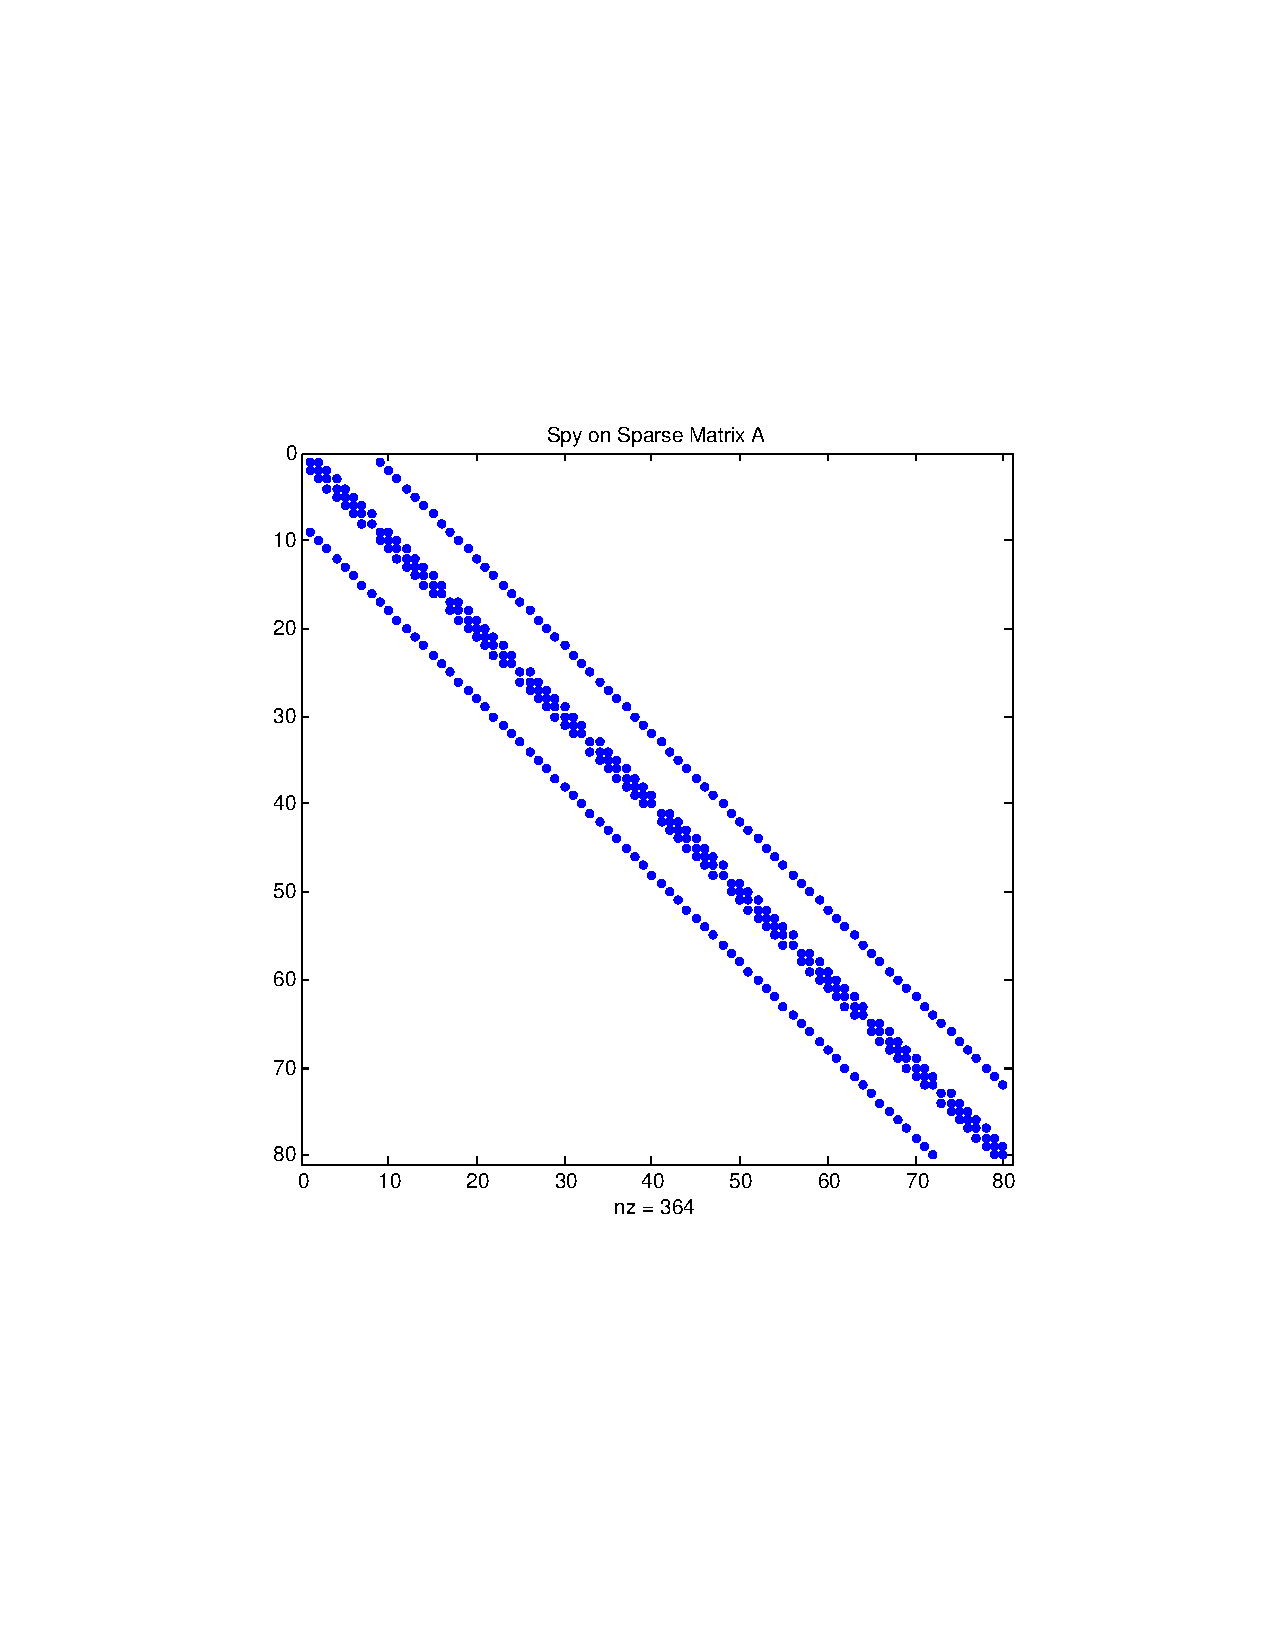
\includegraphics[width=0.5\textwidth]{Fig/FDFDMatrixA.pdf}
  \caption{sparse FDFD matrix $\bA$ for a specific frequency $\omega$. Blue dots denotes the nonzero elements.}
  \label{fig:SparseA}
  \end{figure}
  In order to solve acoustic wave equation in frequency $\omega$, we only have to solve the matrix equation (\ref{awfreq}) where 
  matrix $\bA$ is highly sparse. Matlab has well developed functions to invert the sparse matrix, see Figure \ref{fig:SparseA}. 
  Other than that, when the size of $\bA$ is huge, we recommend a well developed package with Matlab interface called MUMPS (MUltifrontal Massively Parallel sparse direct Solver) to be installed and solved the sparse matrix inversion problem. 
  There are some other properties which made FDFD excels FDTD for our application. Instead of processing the whole data set in time domain,
  we can only solve the wave equation in the important part of spectrum using FDFD, which considerably reduces the volume of the data and makes large-scale problems (e.g., full waveform inversion) feasible. For speed purposes, since the wave equations are independent over frequencies, FDFD can be easily parallelized across frequencies.

An interesting examples is the Green's function, which is the solution of wave equation with an impulse source term. Numerically,
the Green's function cannot be solved accurately with FDTD, because of the impulse function has components in arbitrarily high
frequency. This will bring serve grid dispersion to the numerical solution. However this is not a problem for FDFD. The Green's Function 
$G_{\omega}$ in frequency domain, which solves  
  \begin{equation}
  \frac{\omega^2}{v^2(z, x)}G_{\omega}(z, x) + \nabla^2 G_{\omega}(z, x) = \delta_{\omega}(z-z_0, x-x_0)
  \end{equation}
  is a the solution of (\ref{awfreq}) with the source term $\bff$ contains all one's.
  
  \begin{figure}
  \centering
  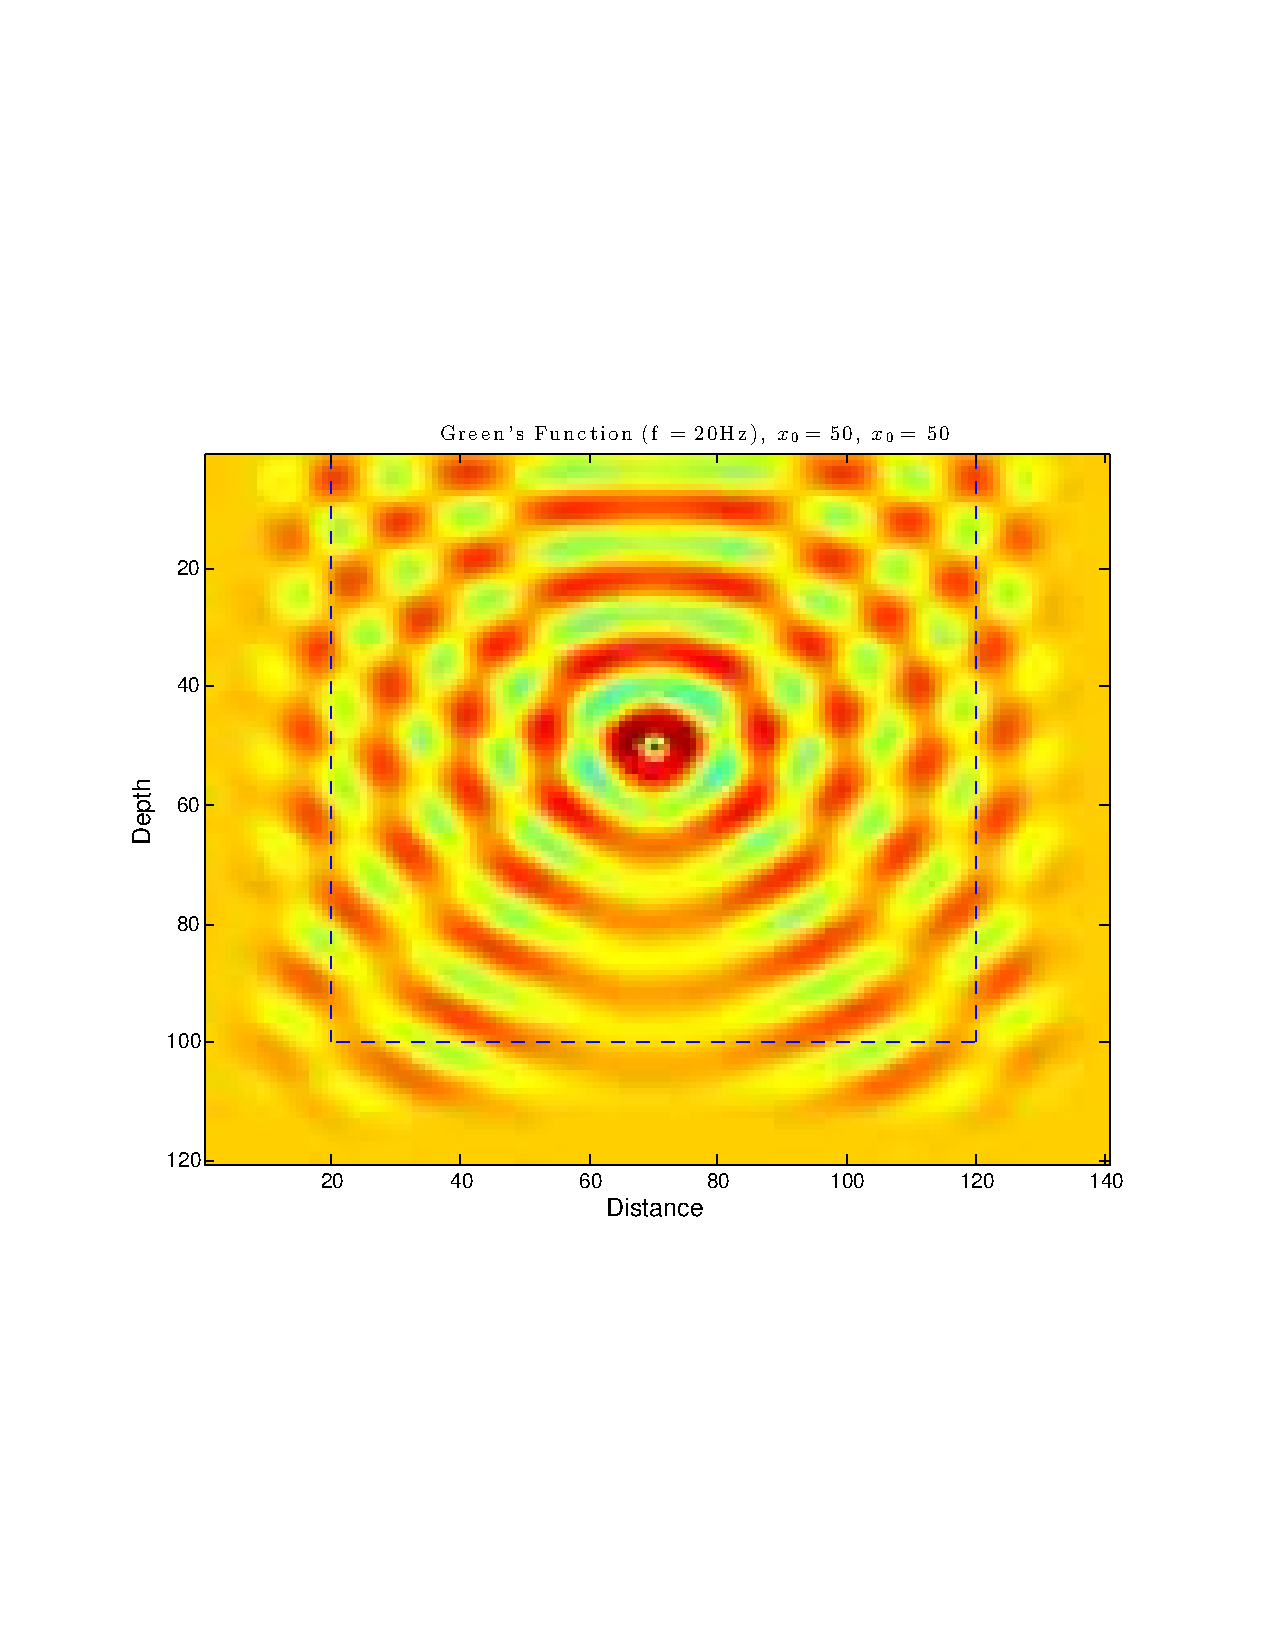
\includegraphics[width=0.5\textwidth]{Fig/GreensFunction.pdf}
  \caption{Real part of the Green's function in frequency domain} 
  \end{figure}


\section{Numerical solution for elastic wave equation}
In the real media, the seismic waves are in the form of elastic waves which are composed of both P-wave and S-wave
\begin{equation}
    \left\{
    \begin{aligned}
    %v_z=\frac{\partial s_z}{\partial t}, \quad &v_x=\frac{\partial s_x}{\partial t}\\
    v_z=v_{zp}+v_{zs}, \quad &v_x=v_{xp}+v_{xs}\\
    \frac{\partial v_{zp}}{\partial t}=\alpha^2 \frac{\partial A}{\partial z}, \quad &\frac{\partial v_{xp}}{\partial t}=\alpha^2 \frac{\partial A}{\partial x}\\
    \frac{\partial v_{zs}}{\partial t}=-\beta^2 \frac{\partial B}{\partial x}, \quad &\frac{\partial v_{xs}}{\partial t}=\beta^2 \frac{\partial B}{\partial z}\\
    A=\frac{\partial s_z}{\partial z}+\frac{\partial s_x}{\partial x}, \quad &B=\frac{\partial s_x}{\partial z}-\frac{\partial s_z}{\partial x}
    %\frac{\partial A}{\partial t}=\frac{\partial v_z}{\partial z}+\frac{\partial v_x}{\partial x}, \quad& \frac{\partial B}{\partial t}=\frac{\partial v_x}{\partial z}-\frac{\partial v_z}{\partial x} 
    \end{aligned}
    \right.
    \end{equation}
    \begin{figure}
    \centering
    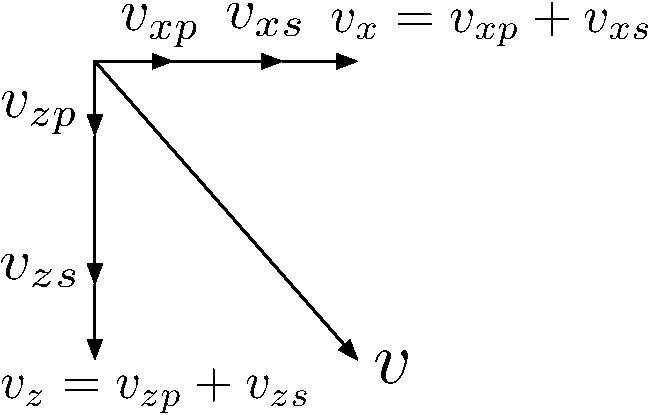
\includegraphics[width=0.5\textwidth]{Fig/EWCoordinates.pdf}
    \caption{Velocity separation}
    \end{figure}
where $(v_z, v_x)$ is the particle velocity field, $v_{up}$ is P-wave field in $u$-direction $(u=x, z)$,
  $v_{us}$ is the S-wave fields in $u$-direction $(u=x, z)$, and $(s_z, s_x)$: particle displacement vector.
  We can see that in this form, we separate the P-wave and S-wave fields in the solution \cite{Che2014}. Since 
  we already split the velocity field into $z$ and $x$ directions, we use a split PML (SPML) for the FDFD. See \texttt{src/fwdTimeSpmlFor2dEw.m}

\section{Migration}
The goal of seismic imaging is to recover the subsurface structures with the recorded seismic data. This imaging process is 
typically computationally intense. There are many imaging algorithms. In SSSI we implemented a few representative ones, such as
Kirchhoff's migration, Reverse Time Migration (RTM), Least square RTM (LSRTM), and Full Waveform Inversion (FWI) in frequency domain.
All methods we implemented in SSSI are prestack.  

\subsection{Kirchhoff's migration}
Let $\bx_r$ be the location of the receiver and $\bx_s$ be the location of the source. 
Then $\bm=(\bx_r+\bx_s)/2$ is the midpoint, and $\bh=(\bx_r-\bx_s)/2$ is the half offset.
The involved derivation of Kirchhoff's migration (see \cite{Sch1978} for details) is omitted here. Only the simple imaging formula 
is given as below
\begin{equation}
I(\xi)=\int_{\Omega_\xi} W(\xi,\bm,\bh)dt(t=t_d(\xi,
\bm,\bh),\bm,\bh)d\bm d\bh,
\end{equation}
where limited region $\Omega_\xi$ is centered around the location $\xi$
in the $m$ plane, called the migration aperture. $t_d=t_s[\bx,\bs,v(z,x,y)]+t_g[\bx,\bg,v(z,x,y)]$.
For reflector $\xi = (z_\xi, x_\xi, y_\xi)$ in 3D and $\xi = (z_\xi, x_\xi)$ in 2D case.

  \begin{figure}
  \centering
  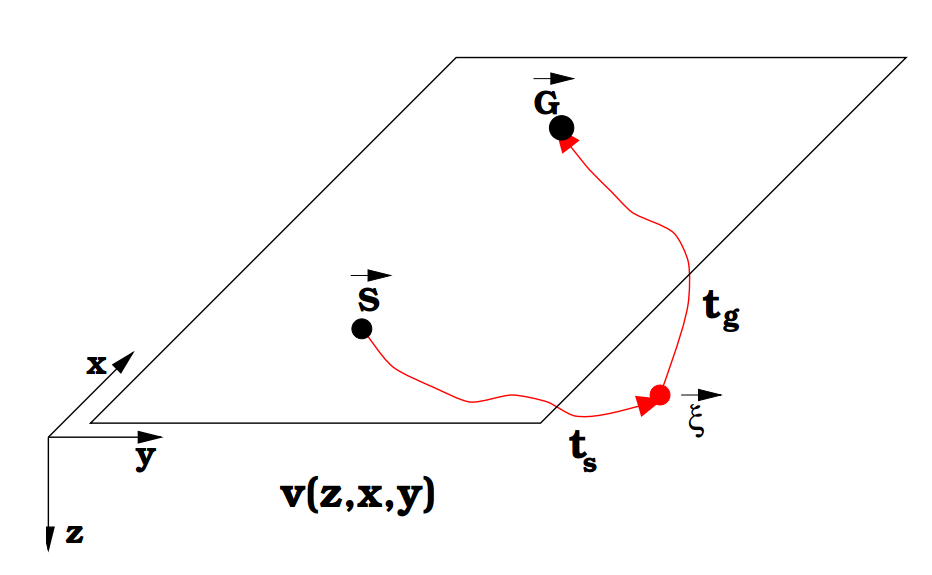
\includegraphics[width=0.5\textwidth]{Fig/tstg.PNG}
  \caption{Reflector, and travel times (adapted from \cite{bio2006})}
  \end{figure}
  
An example of Kirchhoff's migration can be found in \texttt{src/mainKirkCpmlFor2dAw\_ fault.m}, which is 
inherited from a existing package \cite{Koz2011}.
The most important part of Kirchhoff's migration is the computation of travel times $t_s$ and $t_g$.   
These can be done either with \texttt{src/ray2d.m} from \cite{Koz2011}, or
\texttt{src/eikonal2d.m} which solves the 2D Eikonal equation with a fast sweeping method \cite{Zha2004}.
The Eikonal equation can be written as
\begin{equation}
|\nabla T(\bx)| c(\bx)= 1, ~~\bx\in \real^2
\end{equation}
with $T(\bx_s) = 0$ for the source position $\bx_s$. When we solve it in a truncated region, $T(\bx)$ gives the time of first 
arrival in this region.

\subsection{Reverse Time Migration (RTM)}
The Reverse Time Migration (RTM) utilizes received surface data to locate the reflectors. 
RTM has a relatively old origin, however it has not been used routinely until recently because of its
computation expense. RTM has a number of advantages over conventional depth migration methods such as 
handing evanescent energy and no dip limitation \cite{Mcm1983, BayKosAO1983}. In summary, RTM is implemented in three steps. Firstly, 
record forward wave field $p_f(\bx, t; \bx_s)$ through the true velocity model. Secondly, solve the reverse wave field $p_r(\bx, t)$ by the received surface data through the incident model, which is typically a smoothed version of the true model. The second step is equivalent to reverse the recorded traces in time. Then input those traces as source function and solve the wave field. Finally, superposition of above using an imaging condition (chosen from a number existing imaging conditions).

For instance, the imaging condition with cross-correlation is 
\begin{equation}
I(\bx) = \sum_{\bx_s} \frac{\int_0^T p_f(\bx, t; \bx_s)p_r(\bx, t)\mathrm{d}t}{\int_0^T |p_f(\bx, t; \bx_s)|^2\mathrm{d}t + \epsilon^2}.
\end{equation}
The RTM result can be viewed in this video clip
\texttt{https://www.youtube.com/watch?v=lL-UpW-5xms$\&$feature=youtu.be}.

RTM serves the imaging complex structures purposes as a reliable method. However, there are still some distortions caused by RTM crosstalk
artifacts. Mathematically, the migration operator is just a adjoint of the forward modeling operator, it does not minimize the mismatch of the observed and simulated traces. Least Square RTM (LSRTM) introduced by \cite{NemWuAO1999} derives an imaging condition by formulating migration as an inverse problem based on a least-squares misfit function.
  \begin{equation}
  \begin{aligned}
  %\hspace{-20pt}
  J&(\Delta m) = \frac{1}{2} \sum\limits_{\omega} \sum\limits_{\bx_s} \sum\limits_{\bx_r} \left| P_{\omega}^{\text{(sim)}}(\bx_r; \bx_s) - P_{\omega}^{\text{(obs)}}(\bx_r; \bx_s) \right|^2 \\
  &= \frac{1}{2} \sum\limits_{\omega} \sum\limits_{\bx_s} \sum\limits_{\bx_r} \left| \omega^2 F_{\omega}(\bx_s) \sum\limits_{\bx}\Delta m(\bx)G_{\omega}(\bx; \bx_s)G_{\omega}(\bx_r; \bx) \right.\\&\left.- \delta P_{\omega}(\bx_r; \bx_s) \right|^2\\
  &= \frac{1}{2} \left\| \bL\Delta m - \delta\bP_{\omega}\right\|_2^2,
  \end{aligned}
  \end{equation}
  where $\Delta m$ is the module perturbation (roughly saying, the reflectors), $\bL$ is the forward modeling operator. The superscript (sim) means simulated results and (obs) means
  observed. The optimized model perturbation by Gauss-Newton method
    \begin{equation}
    \Delta m^{\text{(opt)}} = \underbrace{\left( \bL^{\dag}\bL \right)^{-1}}_{\text{Preconditioner}} \underbrace{\bL^{\dag} \delta\bP_{\omega}}_{\text{RTM}}.
    \end{equation}
    Apparently, LSRTM is the simply a preconditioned RTM migration.  



\begin{figure}
\centering
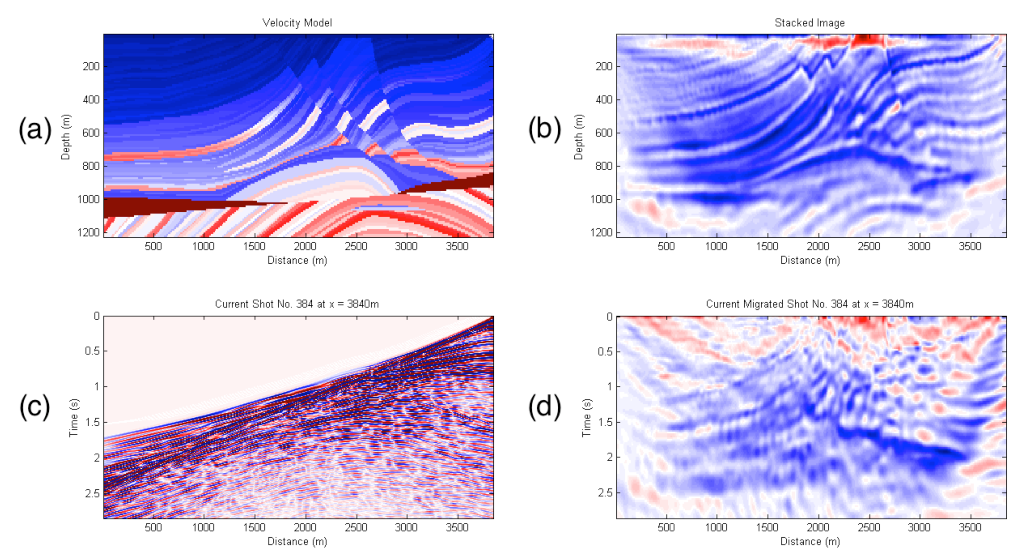
\includegraphics[width=1\textwidth]{Fig/MarmousiRTM.pdf}
\caption{RTM results. (a) Marmousi model, (b) accumulated RTM result; (c) a sample shot record; (d) migrated result of the sample shot. The parameters settings are 15 Hz (center frequency) Ricker wavelet, 384 sensors, 384 shots, grid size $122 \times 384$, $\Delta z = \Delta x = 24m$.}
\end{figure}





\section{Full Waveform Inversion (FWI) in frequency domain}
The migration operator should have a incident model (usually a smoothed version of the true model) as an input. However, an accurate initial velocity model is not always available. The Full Waveform Inversion (FWI) (see \cite{VirOpe2009} as an overview) provides flexibility of updating the initial model iteratively.  $J(\Delta m)$ can be optimized by more approaches: conjugate-gradient, quasi-Newton, etc.

\begin{algorithm}[H]
\begin{algorithmic}[1]
\WHILE{$m(\bx)$ is not converged}
\STATE Generate Green's functions at each shot and receiver for $\bL$
\STATE Generate scattering wave field $\delta\bP_{\omega}= \bP_{\omega}^{\text{(obs)}} - \bG_{\omega}(m)\bF_{\omega}$
\STATE $\Delta m^{\text{(opt)}} = \arg\min J(\Delta m) = \arg\min \frac{1}{2} \left\| \bL\Delta m - \delta\bP_{\omega}\right\|_2^2$
\STATE $m \leftarrow m + \Delta m$
\ENDWHILE
\end{algorithmic}
\caption{Full Waveform Inversion}
\end{algorithm}


\bibliographystyle{ieeetr}
\bibliography{UserGuide}






\end{document}
